\chapter{Déroulement du programme}

    \section{Lancement du programme et timeout}
    
    Au lancement du programme scheduler, un temps d'expiration (timeout) est lancé. Passé ce timeout, le programme quittera automatiquement. Le timeout est de 60 secondes au lancement du programme, et est relancé à chaque tâche reçue par le scheduler pour la valeur du timeout de la tâche entrée par l'utilisateur auquel nous additionnons 60 secondes. L'utilisateur a donc en moyenne une minute pour interagir avec le programme avant que celui-ci ne quitte.
    Si le programme scheduler quitte, le relancer suffira pour de nouveau interagir avec le programme client, même si celui-ci n'a pas été fermé.

    \section{Remplissage de la file de message}
    
    Afin que l'ordonnanceur puisse travailler, il faut tout d'abord remplir la file avec des tâches à consommer. Pour cela, exécuter le programme en mode client :
    
    \begin{verbatim}
        $ ./Scheduler --client
    \end{verbatim}
    
    Puis choisissez le mode d'envoi des messages que vous souhaitez. Vous pouvez laisser le client ouvert et continuer à envoyer des tâches dans la file pendant l'exécution de l'ordonnanceur. Ne pas oublier d'ouvrir un scheduler :
    
    \begin{verbatim}
        $ ./Scheduler --sequential
        $ ./Scheduler --parallel
    \end{verbatim}

    

    \section{Workflow}
    
    \vfill
    \begin{figure}[!b]
        \centerline {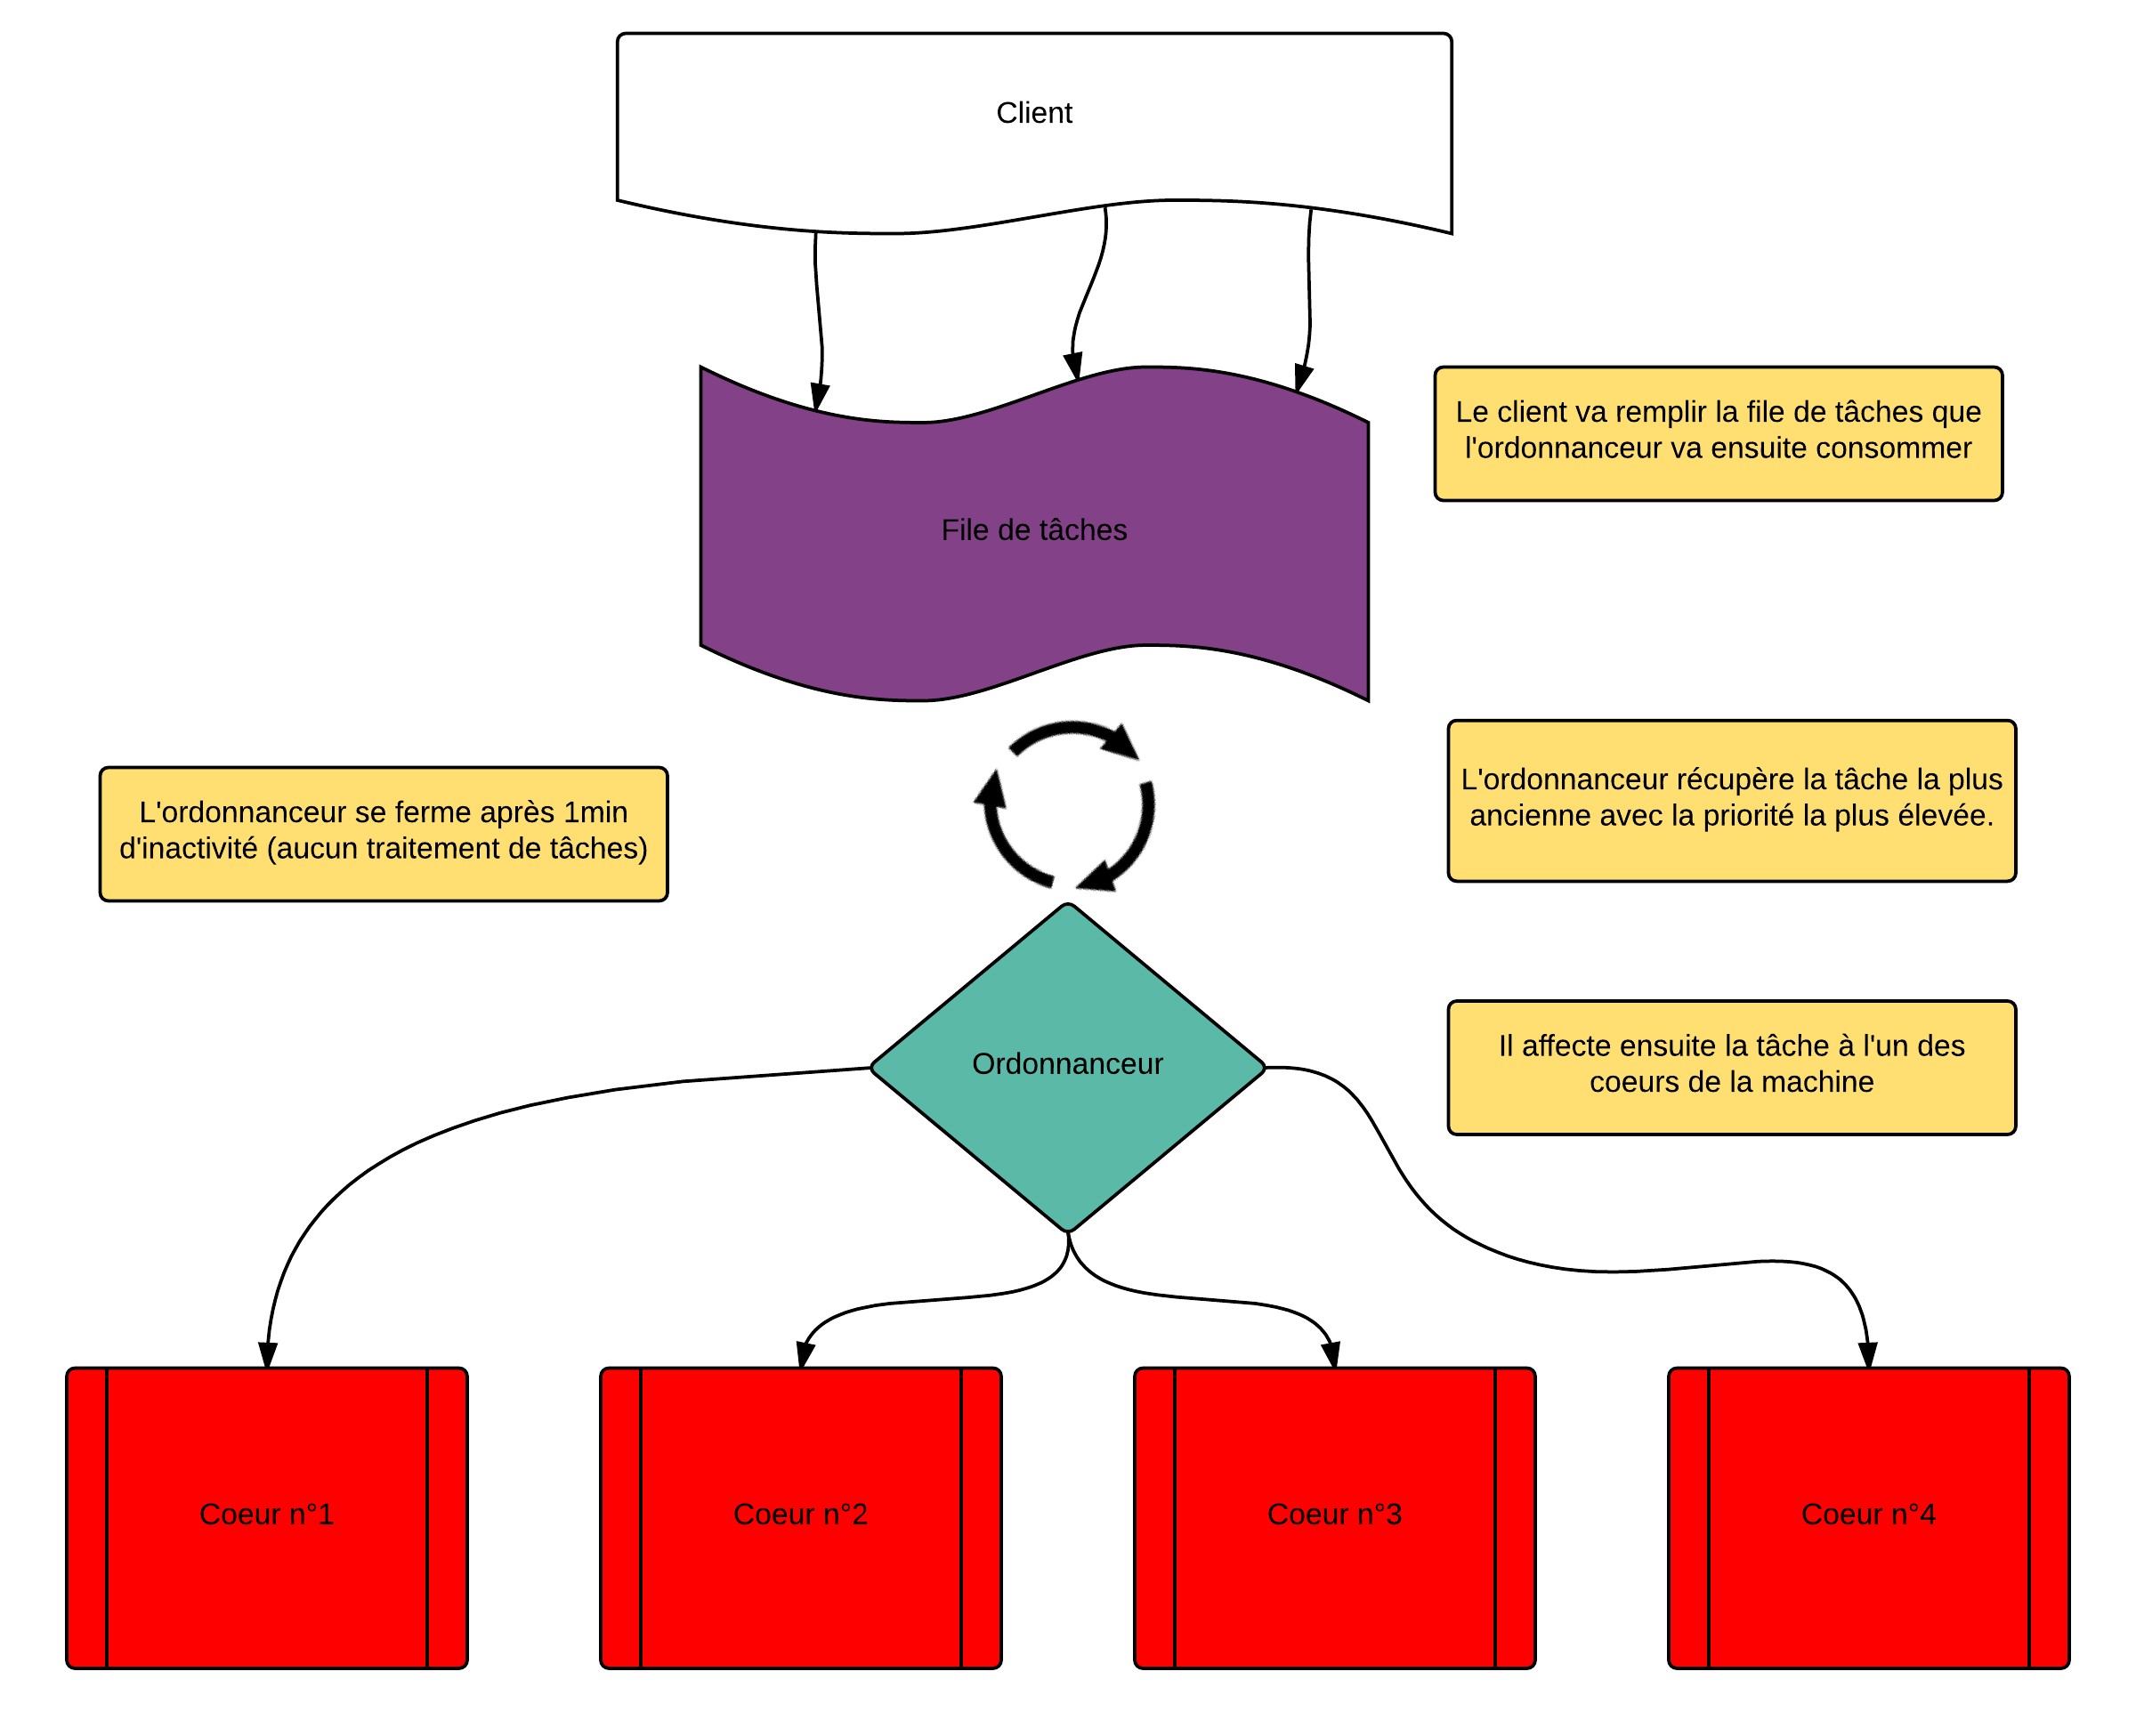
\includegraphics[scale=0.22]{workflow.png}}
        \caption{Workflow (happy path) de notre programme}
        \label{Workflow (happy path) de notre programme}
    \end{figure}